\documentclass[pdftex,11pt]{article}
\usepackage{url}
\usepackage{graphicx}
\usepackage{hyperref}
\usepackage{latexsym,amssymb}
\usepackage{amssymb,amsmath}
\usepackage{color}
\input{../../vrac/rgb.tex}

\usepackage[english]{babel}
\usepackage{array}
\usepackage{multirow} 

\hypersetup{
pdftitle={Langou :: Sauer EX.0.1.1 (answer)},
pdfauthor={Julien Langou}, 
} 

\setlength{\oddsidemargin}{-0.5in}
\setlength{\evensidemargin}{-0.5in}

\setlength{\textwidth}{7.4in}
\setlength{\textheight}{10.0in}

\setlength{\topmargin}{-0.75in}
\setlength{\headheight}{0pt}
\setlength{\headsep}{0pt}

\setlength{\parindent}{0pt}

\begin{document}

\thispagestyle{empty}
\pagestyle{empty}
\renewcommand{\theenumi}{\alph{enumi}}

%
\framebox{
\begin{minipage}{\textwidth}
{\tiny
{\bf Copyright (C) 2018, 2012, 2016 by Pearson Education Inc. All Rights Reserved,}
please visit \url{www.pearsoned.com/permissions/}.}
%{\bf Copyright (C) 2018, 2012, 2016 by Pearson Education Inc. All Rights Reserved.}
%Printed in the United States of America.
%This publication is protected by copyright, and permission should be obatined from the 
%publisher prior to any prohibted reproduction, storage in retrieval system, or 
%transmission in any form of by any means, electronic, mechanical, photocopying, recording, 
%or otherwise. For information regarding permissions, request forms and the appropriate 
%contacts within the Pearson Education Global Rights \& Permissions department, 
%please visit \url{www.pearsoned.com/permissions/}.}
%
\end{minipage}}




\framebox{
\begin{minipage}{\textwidth}
%\textbf{Sauer EX.0.1.1}\hfill\textbf{Langou}\\\\
\textbf{EX.0.1.1, Sauer}\\\\
Rewrite the following polynomials in nested form. 
Evaluate with and without nested form at $x=1/3$.
\begin{enumerate}
\item $ p(x) =  6x^4 + x^3 + 5x^2 + x + 1$
\item $ p(x) = -3x^4 + 4x^3 + 5x^2 - 5x + 1$
\item $ p(x) =  2x^4 + x^3 - x^2 + 1$
\end{enumerate}
\end{minipage}}

\vspace*{.7cm}

\framebox{
\begin{minipage}{\textwidth}
{\tiny
{\bf Copyright (c) 2021, Julien Langou. All rights reserved,}
please visit \url{https://creativecommons.org/licenses/by/4.0/}.}
\end{minipage}}
\vspace*{.2cm}

\textbf{EX.0.1.1, Sauer, solution, Langou}\\

See as well the {\color{blue}\href{https://colab.research.google.com/drive/1arK76rXisavmsbDRAj_L_vk6mi2unRtq?usp=sharing}{Colaboratory Jupyter Notebook}}.\\

In nested form,
\begin{enumerate}
\item $ p(x) = 6x^4 + x^3 + 5x^2 + x + 1 = ( (6x + 1 ) x + 5 ) x + 1 ) x + 1 $
\item $ p(x) = -3x^4 + 4x^3 + 5x^2 - 5x + 1 = ( ( -3x + 4 ) x + 5 ) x - 5 ) x + 1 $
\item $ p(x) =  2x^4 + x^3 - x^2 + 1 = ( ( 2x + 1) x - 1) x^2 + 1   $
\end{enumerate}

And we can check that, using either standard form or nested form to evaluate the polynomial at $x=\frac13$, 
we get
\begin{enumerate}

\item $ p(\frac{1}{3}) = 2 $\\
\framebox{\begin{minipage}{0.5\textwidth}
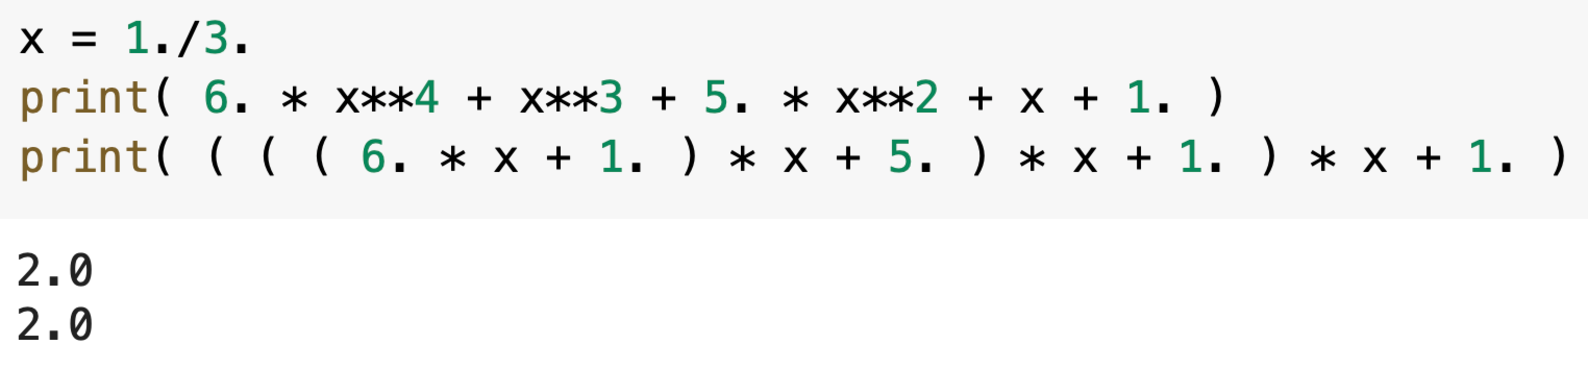
\includegraphics[width=\textwidth]{exercise_ex_0_1_01________sauer____sol_langou__parta.pdf}
\end{minipage}}

\item $ p(\frac{1}{3}) = 0 $\\
\framebox{\begin{minipage}{0.5\textwidth}
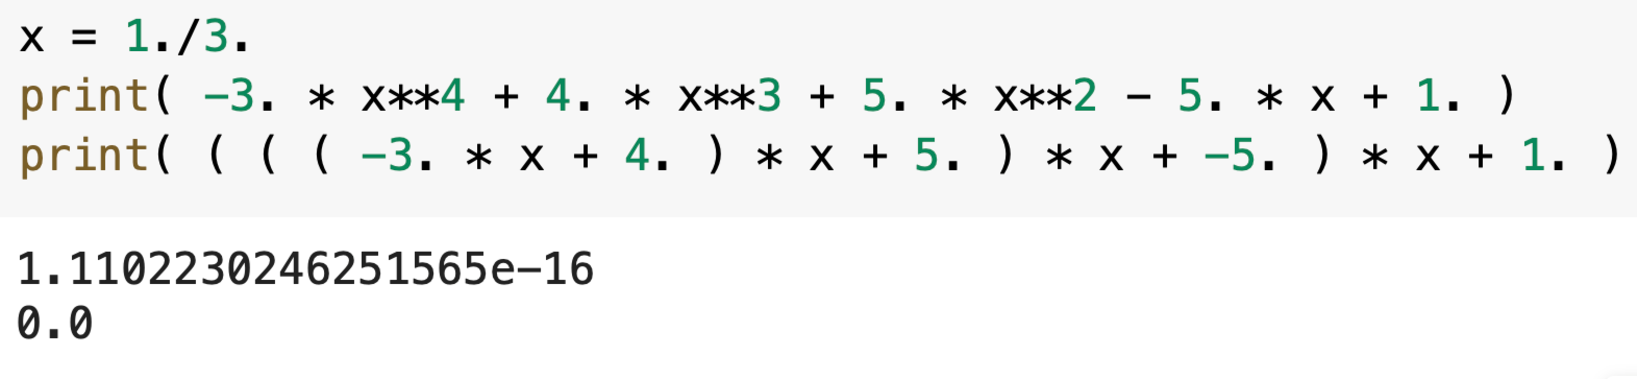
\includegraphics[width=\textwidth]{exercise_ex_0_1_01________sauer____sol_langou__partb.pdf}
\end{minipage}}


\item $ p(\frac{1}{3}) =  \frac{77}{81}   $\\
\framebox{\begin{minipage}{0.5\textwidth}
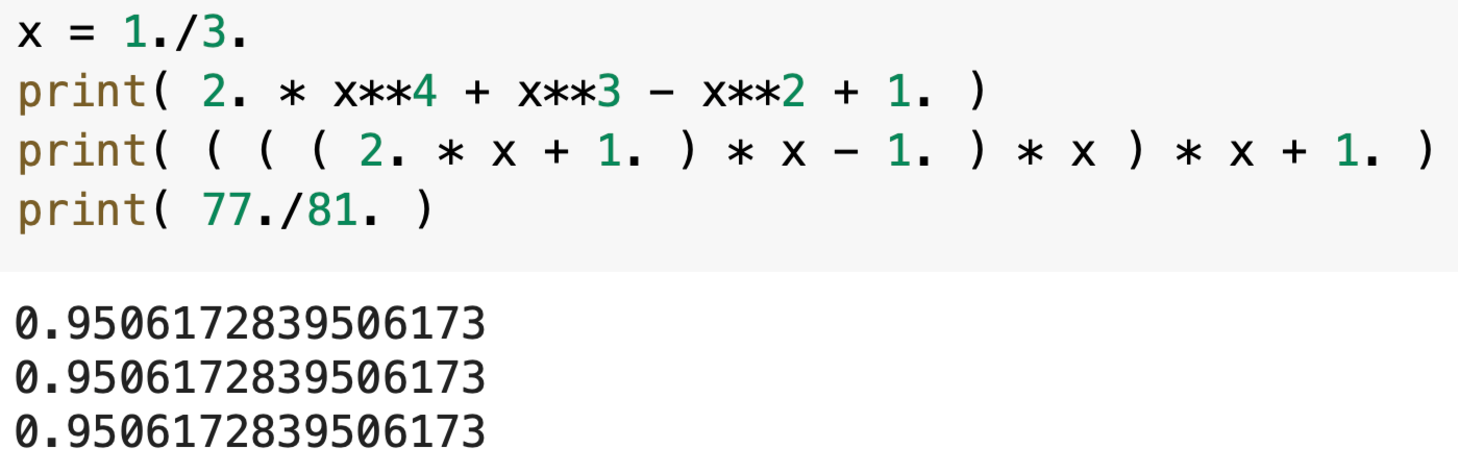
\includegraphics[width=\textwidth]{exercise_ex_0_1_01________sauer____sol_langou__partc.pdf}
\end{minipage}}

\end{enumerate}


\end{document}
